\documentclass[12pt]{article}
\usepackage{amsmath,amssymb,bm}
\usepackage{booktabs, tabularx}
\usepackage{graphicx}
\usepackage{enumerate}
\usepackage{natbib}
\usepackage{hyperref}
\usepackage{url} % not crucial - just used below for the URL 

\graphicspath{{./figures/}{.}{./terms/}}
\usepackage{pstricks}

%\pdfminorversion=4
% NOTE: To produce blinded version, replace "0" with "1" below.
\newcommand{\blind}{0}

% DON'T change margins - should be 1 inch all around.
\addtolength{\oddsidemargin}{-.5in}%
\addtolength{\evensidemargin}{-1in}%
\addtolength{\textwidth}{1in}%
\addtolength{\textheight}{1.7in}%
\addtolength{\topmargin}{-1in}%


% DELETED!
% DELETED!
% DELETED!
% DELETED!
% DELETED!

% DELETED!
\newcommand{\sufstats}[1]{\bm{g}\left(#1\right)}
\renewcommand{\exp}[1]{\mbox{exp}\left\{#1\right\}}
\renewcommand{\log}[1]{\mbox{log}\left\{#1\right\}}
\newcommand{\transpose}[1]{{#1}^{\bm{t}}} 
\renewcommand{\t}[1]{\transpose{#1}}

\newcommand{\s}[1]{\sufstats{#1}}
\newcommand{\SUFF}{\bm{S}}
\newcommand{\Suff}{\bm{G}}
\newcommand{\suff}{\bm{g}}

\newcommand{\coef}{\bm{\theta}}
\newcommand{\weight}{\bm{w}}
\newcommand{\Weight}{\bm{W}}

% Objects
% DELETED!
% DELETED!
\newcommand{\Graph}{\bm{Y}}
\newcommand{\graph}{\bm{y}}
\newcommand{\g}{\graph}
\newcommand{\GRAPH}{\mathcal{Y}}
\newcommand{\Adjmat}{A}
\newcommand{\adjmat}{a}
\newcommand{\ADJMAT}{\bm{A}}

\newcommand{\INDEPVAR}{\bm{X}}
\newcommand{\Indepvar}{X}
\newcommand{\indepvar}{x}

\newcommand{\normconst}{\kappa_{\GRAPH}\left(\coef\right)}


% \bibliography{bibliography.bib}

\def\ergmito{ERGM\textit{ito}}
\def\ergmitos{\ergmito{}\textit{s}}
% Mathematical functions
\newcommand{\isone}[1]{{\boldsymbol{1}\left( #1 \right)}}
\newcommand{\f}[1]{{f\left(#1\right) }}

% Define a command with an optional argument

% \usepackage[]{xparse}
% \NewDocumentCommand{\Prcond}{m m o}{
%   \IfNoValueTF{#3}{%
%   {\mbox{Pr}\left(#1;\;#2\right)} %
%   }{%
%   {\mbox{Pr}_{#3}\left(#1;\;#2\right)} %
%   }
% }

\renewcommand{\Pr}[1]{{\mbox{Pr}_{\GRAPH,\coef}\left(#1\right) }}
\newcommand{\Prcond}[2]{%
  {\mbox{Pr}_{\GRAPH,\coef}\left(#1\left|\;#2\right.\right)}%
  }
\newcommand{\fcond}[2]{{f\left(#1|#2\right) }}
\newcommand{\Expected}[1]{{\mathbb{E}\left\{#1\right\}}}
\newcommand{\ExpectedCond}[2]{{\mathbb{E}\left\{#1\vphantom{#2}\right|\left.\vphantom{#1}#2\right\}}}
\renewcommand{\exp}[1]{\mbox{exp}\left\{#1\right\}}

\newcommand{\Likelihood}[2]{\text{L}\left(#1 \left|\vphantom{#1}#2\right.\right)}

\newcommand{\loglik}[1]{l\left(#1\right)}

\begin{document}

%\bibliographystyle{natbib}

\def\spacingset#1{\renewcommand{\baselinestretch}%
{#1}\small\normalsize} \spacingset{1}


%%%%%%%%%%%%%%%%%%%%%%%%%%%%%%%%%%%%%%%%%%%%%%%%%%%%%%%%%%%%%%%%%%%%%%%%%%%%%%

\def\blind{1}

\if1\blind
{
  \title{\bf Power and multicollinearity in small networks: A discussion of\\``Tale of Two Datasets: Representativeness
  and Generalisability of Inference for Samples of Networks'' by \citeauthor*{krivitskyTaleTwoDatasets2022}}
  \author{George G. Vega Yon\hspace{.2cm}\\%
    Division of Epidemiology, University of Utah
    }
  \maketitle
} \fi

\if0\blind
{ 
  \bigskip
  \bigskip
  \bigskip
  \begin{center}
    {\LARGE\bf A comment on\\``Tale of Two Datasets: Representativeness
    and Generalisability of Inference for Samples of Networks'' by \citeauthor*{krivitskyTaleTwoDatasets2022}}
\end{center}
  \medskip
} \fi

\spacingset{1.9} % DON'T change the spacing!

The recent work by \citeauthor*{krivitskyTaleTwoDatasets2022} [KCH] provides an important new contribution to the Exponential-Family Random Graph [ERG] Models, a start-to-finish approach to dealing with multi-network ERGMs. Although multi-network ERGMs have been around for a while (mostly in the form of block-diagonal models and multi-level ERGMs, see \cite{duxburyScalingBiasPooled2023,wangExponentialRandomGraph2013, slaughterMultilevelModelsSocial2016}), not much care has been given to the estimation and post-estimation steps. In their paper, \citeauthor*{krivitskyTaleTwoDatasets2022} give a detailed layout of how to build, estimate, and analyze multi-ERG models with heterogeneous data sources. In this comment, I will focus on two issues the authors did not discuss: sample size requirements and multicollinearity, the latter regarding small networks. 


\section{Sample size requirements in ERGMs}

Samples of multiple networks are becoming increasingly common \citep{yonExponentialRandomGraph2021,krivitskyTaleTwoDatasets2022, duxburyScalingBiasPooled2023}. Because of the complexity of ERGMs, power analysis (as in the required sample size for doing inference) has not been discussed in much of the literature other than in brief mentions (as in \cite{yonExponentialRandomGraph2021}). In this scenario, it is natural to start thinking about power analysis in ERGMs, especially in the case of small networks like those featured in egocentric studies, as, from the financial point of view, small networks are easier to collect. In ERG models, power analysis has two different parameters to pick: the network size and the number of networks. 

\bigskip

\noindent \textbf{Network size}. Size for network studies, defined as the number of nodes to include in an ERG model, has two sides: network boundaries (as ``finite'' versus ``continuous'' in \cite{buttsRevisitingFoundationsNetwork2009}) and statistical inference (as in projectivity). Many times the studied network has a well-defined boundary, for example, team networks and school friends. In such a scenario, surveying the entire network is completely feasible, so the question ``How many nodes to survey?'' is irrelevant. On the other hand, when the network boundaries are not well defined (like in a citation network), or the number of nodes in the network is large, ``How many nodes are needed?'' for statistical inference becomes relevant. In oversimplified terms, projectivity in our context refers to the validity of inference on a subset of the complete graph. Although many ERGMs are not projective, it has been shown that projectivity is not a necessary condition for consistency in likelihood-based inference \citep{schweinbergerNoteRoleProjectivity2017, schweinbergerExponentialFamilyModelsRandom2020}. In the case of KCH, since they deal with networks within households, boundaries are well defined, so the relevant size question is ``How many households to survey?''.
% Add a couple of sentences concluding this part
 
\bigskip

\noindent\textbf{Number of networks}. Here, the number of networks is akin to sample size in traditional statistical analyses. From the practical point of view, researchers' capacity to generate data as that featured in \citeauthor*{krivitskyTaleTwoDatasets2022}'s is tightly related to funding opportunities. Having a way of justifying the number of networks required in research projects is highly relevant.

As high computational power is increasingly accessible, one possible approach is to design a framework for power analysis in pooled ERGMs via simulation studies. For example, scientists exploring the role of gender in small teams could use observed data on density to estimate the number of networks needed to detect a given effect size using conditional ERGMs.  Using the same notation as in \cite{krivitskyTaleTwoDatasets2022}, the conditional ERG probability mass function [PMF] given the $l$-th statistic, $\s{\g}_l = s_l$, can be calculated as follows:

\begin{align}
\notag\Prcond{\Graph = \g}{\s{\g}_l = s_l}  & = \frac{%
	\Pr{\s{\Graph}_{-l} = \s{\g}_{-l}, \s{\g}_l = s_l}
}{%
	\sum_{\g'\in\GRAPH:\s{\g'}_l = s_l}\Pr{\s{\Graph} = \g'}%
} \\ & =  %
\frac{%
	\exp{\t{\coef_{-l}}\s{\g}_{-l}}
}{%
	\normconst_{-l}
}, \label{eq:conditional-ergm}
\end{align}


\noindent where $\s{\g}_l$ and $\coef_l$ are the $l$-th element of $\s{\g}$ and $\coef$ respectively, $\s{\g}_{-l}$ and $\coef_{-l}$ are their complement, and $\normconst_{-l} = \sum_{\g' \in \GRAPH: \s{\g'}_l = s_l}\exp{\t{\coef_{-l}}\s{\g'}_{-l}}$ is the normalizing constant. In other words, once we condition on the $l$-th sufficient statistic, the PMF becomes invariant to the value of $\coef_l$. Using the conditional distribution, we could simulate networks with a given edge count (which drives an important part of the ERG probability) and infer the required sample size. For instance, in a study where gender homophily in networks of size 8 is the main focus, and assuming an effect size of $\coef_{\mbox{homophily}} = 2$ and edge count of 20 (\textit{i.e.}, a density of $(2\times 20)/(8 \times 7) \approx 0.71$), we could approximate the required sample size in the following fashion:

\begin{enumerate}
  \item For each $n \in N \equiv \{10, 20, \dots\}$, do:
  \begin{enumerate}
    \item With Equation \eqref{eq:conditional-ergm}, use MCMC simulate $1,000$ sets of $n$ networks of size 8 and 20 ties.
    \item For each set, fit a conditional ERGM to estimate $\hat\coef_{\mbox{homophily}}$, and generate the indicator variable $p_{n, i}$ equal to one if the estimate is significant at the 95\% level.
    \item The empirical power for $n$ is equal to $p_n \equiv \frac{1}{1,000}\sum_{i}p_{n, i}$.
  \end{enumerate}
  \item Once we have computed the sequence $\{p_{10}, p_{20}, \dots\}$, we can fit a linear model to estimate the sample size as a function of the power, \textit{e.g.}, $n = \beta_0 + \beta_1 p_n + \beta_2 p_n^2 + \varepsilon$.
  \item With the previous model in hand, we can estimate the sample size required to detect a given effect size with a given power.
\end{enumerate}

Again, it is worth emphasizing that, by fixing the number of observed ties (edge count,) we do not need to assume a value for its corresponding parameter; greatly simplifying the analysis. With more and more data sources featuring multiple networks as in \cite{krivitskyTaleTwoDatasets2022}, it is important to have a way of justifying the number of networks needed to detect a given effect size. This is especially critical from the research funding point of view, as such information can be critical to explaining the financial resources required for multi-network studies.

\section{Collinearity in small networks}

Since most of the statistics used in ERG models are by construction function of the number of ties in the network, the problem of collinearity is embedded in ERGMs. If we learned one thing from \cite*{duxburyDiagnosingMulticollinearityExponential2021}'s large simulation study is that traditional measurements of collinearity are completely off in network models, with the Variance Inflation Factor [VIF] surpassing the rule of thumb of 10 by orders of magnitude in most cases.

As a proof of concept, I have selected four statistics that are commonly used in the ERGM literature, including the \textit{Edge count} term, to analyze how these are interrelated using \eqref{eq:conditional-ergm}; these statistics are (a) \textit{Number of Mutual Ties}, $\sum_{i\neq j}y_{ij}y_{ji}$; (b) \textit{Number of Transitive Triads} (transitivity), $\sum_{i\neq j\neq k}y_{ij}y_{jk}y_{ik}$; (c) \textit{Number of Homophilic Ties}, $\sum_{i\neq j}y_{ij}\mathbf{1}\left(x_i=x_j\right)$; (d) and \textit{Attribute-Receiver effect}, $\sum_{i\neq j}y_{ij}x_j$, with the latter two using the binary nodal attribute \textit{Gender}, $x_i$, which equals to one if the $i$-th node is female and zero otherwise. All calculations and figures were done using R version 4.3.1 \citep{R}, the R packages \textbf{ergm} \citep{hunterErgmPackageFit2008,handcockErgmFitSimulate2023,krivitskyErgm4NewFeatures2023}, \textbf{ergmito} \citep{ergmito,yonExponentialRandomGraph2021}, and \textbf{ggplot2} \citep{ggplot2}.

\bigskip

\noindent \textbf{In-sample, not out-of-sample predictive power}. Figure \ref{fig:condprob-ttriads} depicts the 95\% Confidence Interval [CI] (shaded area), and fiftieth-percentile (red dashed-lines), of the number of transitive triads (y-axis) when conditioning on the other statistics (x-axis), while at the same time, either assuming that the number of transitive triads has no effect in the data-generating-process [DGP], ($\coef_{\mbox{ttriad}} = 0$), first-row of figures, or on the contrary, assuming that the term is part of the DGP, (fixing $\coef_{\mbox{ttriad}}= 1$), second-row of figures. The baseline graph used to calculate these statistics was a directed network of size five with the gender attribute equal to $(0,0,0,1,1)$, \textit{i.e.}, three males and two females. Figure~\ref{fig:maxout-gof} illustrates three possible configurations, particularly the required arrangement (number and assignment of ties) needed for the analyzed sufficient statistics to reach their maximum values.

\begin{figure}[]
    \centering
    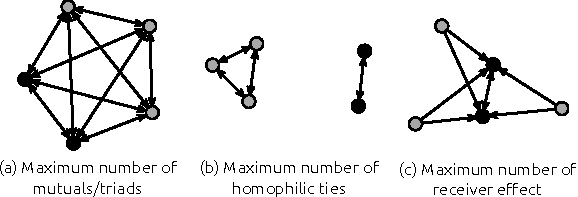
\includegraphics[width = .7\linewidth]{figures/max-out-stats.pdf}
    \caption[Examples of Networks with the maximum observed counts]{\textbf{Networks with maximum observed counts.} All three networks have five vertices composed of two females (black vertices) and three males (gray vertices).
    Network (a) shows the required set of ties to reach the maximum value of \textit{Mutuals} and \textit{Transitive Triads}, which coincides with a fully connected graph, containing $(5\times 4)/2 = 10$ mutual ties and $5 \times 4 \times 3 = 60$ transitive triads.
    Graphs (b) and (c) show the required configuration to maximize the number of \textit{Gender-Homophily} and \textit{Gender-Receiver Effect}, each equal to $3\times 2 + 2\times 1 = 8$ and $4 + 4 = 8$, respectively.}
    \label{fig:maxout-gof}
\end{figure}

As seen in Figure~\ref{fig:condprob-ttriads}, the CI for the expected number of transitive triads is generally very narrow. Since this statistic reflects relatively high-order structures (because more ties are involved), its range of possible values given the number of edge counts or mutual ties is highly constrained. Neither \textit{Gender-Homophily} nor \textit{Gender-Receiver Effect} seem to be very related to transitivity; yet, as $\coef_{\mbox{ttriad}}: 0\to 1$, all four conditioning statistics become very good at predicting the number of transitive triads in the graph. Furthermore, the VIF of transitivity as a function of mutual ties is almost 5,000 and the correlation between those two is almost 1.0. This would not pass the recommendations made by \citeauthor*{duxburyDiagnosingMulticollinearityExponential2021}, who suggests that ERGM VIFs above 150 should be concerning.

% %Checkout pages 15/16 footnote of the SERGM paper

\begin{figure}[]
    \centering
    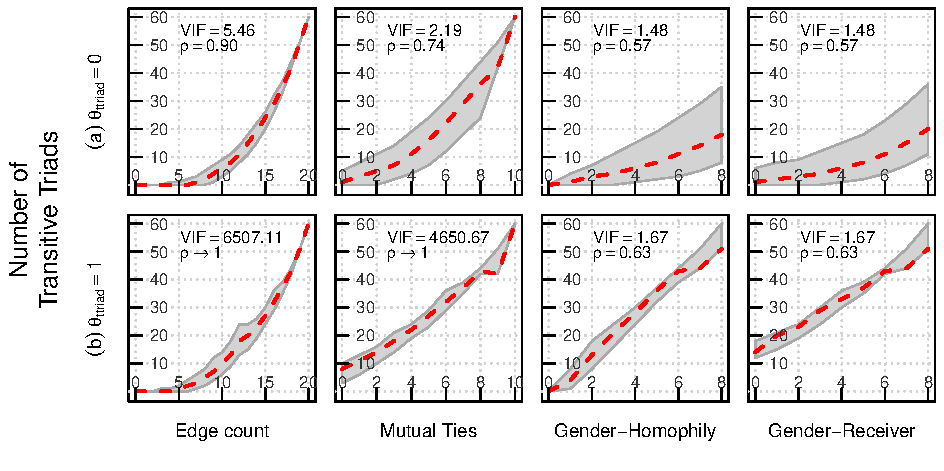
\includegraphics[width = .85\linewidth]{figures/conditional-prob-ttriad.pdf}
    \caption[Conditional Distribution of the Transitive Triads Sufficient Statistic]{Conditional distribution of the number of transitive triads sufficient statistic. Row \textbf{(a)} shows the distribution under the Bernoulli model; this is, the parameter of transitivity is set to zero, whereas row \textbf{(b)} shows the distribution of the statistic assuming $\coef_{ttriad} = 1$.}
    \label{fig:condprob-ttriads}
\end{figure}

Concerning the relatively poor predictive power of the \textit{Gender-Homophily} and \textit{Gender-Receiver Effect} sufficient statistics, part of this could be because they reach their maximum value very quickly (see Figure~\ref{fig:maxout-gof}), as in our case they only needed eight out of the 20 possible ties to find a configuration that had the maximum number of either of the statistics. This implies that if we observe a homophily/attribute-receiver count equal to 6, 7, or 8, there could be any number of ties between 6 to 18, 7 to 19, or 8 to 20, respectively.

\noindent \textbf{Collinearity}. Following \cite{duxburyDiagnosingMulticollinearityExponential2021}, I calculated the VIF and the correlation between transitive triads and mutual ties for networks of size five (with KCH networks' between 2 and 8 nodes) across various combinations of model parameters. The results are shown in Figure~\ref{fig:vif-cor}. Like in the previous figure, instead of simulating networks, we use the full support of the model.

\begin{figure}
  \begin{minipage}
    {.5\linewidth}
    \centering
    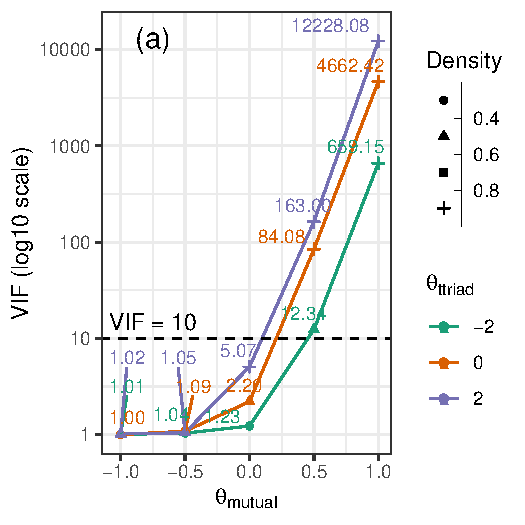
\includegraphics[width = 1\linewidth]{figures/vif-n=5.pdf}
  \end{minipage}
  \begin{minipage}
    {.5\linewidth}
    \centering
    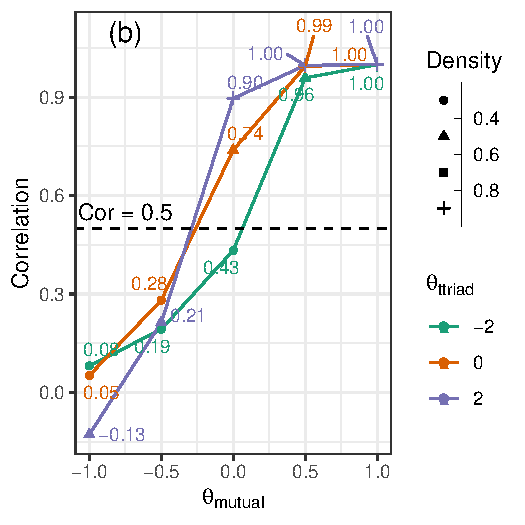
\includegraphics[width = 1\linewidth]{figures/cor-n=5.pdf}
  \end{minipage}
  \caption[]{\textbf{VIF and correlation between terms for networks of size 5}. Each point represents the value of the VIF/Correlation for the given combination of model parameters. The VIF/Correlation is calculated using the full support of the model; in other words, instead of using simulated values as in \cite{duxburyDiagnosingMulticollinearityExponential2021}, we use the full support of the model. The reported network density is the average density of the full support of the model.}
  \label{fig:vif-cor}
\end{figure}

From the figure, it is apparent that, as suggested by \citeauthor{duxburyDiagnosingMulticollinearityExponential2021}, the VIF rule of thumb using VIF=10 to dictate collinearity is quickly reached in ERGMs. In my example, as soon as $\coef_{\mbox{mutual}}$ is above 0.5, the VIF is already above 10. Moreover, in a model with $\coef_{\mbox{ttriad}} = 0$ and $\coef_{\mbox{mutual}} = 1$, the VIF is about 4,600, and the correlation between the two network statistics reaches almost 1.0; a severe level of collinearity between these two terms. Notably, since in \cite{krivitskyTaleTwoDatasets2022} the average network density was 0.93 and 0.73 for the \textit{H} (\textit{household}) and \textit{E} (\textit{egocentric}) respectively, it is to expect to observe severe VIF and correlation as that observed here.

Although VIFs and correlation greatly matter across linear models, after this experiment, \citeauthor*{duxburyDiagnosingMulticollinearityExponential2021}'s work, and \citeauthor*{krivitskyTaleTwoDatasets2022}, it is not conclusive how much it matters for ERGMs. After all, ERGMs are, by construction, endogenous.


% \bigskip
% \begin{center}
% {\large\bf SUPPLEMENTARY MATERIAL}
% \end{center}

% \begin{description}

% \item[Title:] Brief description. (file type)

% \item[R-package for  MYNEW routine:] R-package MYNEW containing code to perform the diagnostic methods described in the article. The package also contains all datasets used as examples in the article. (GNU zipped tar file)
 
% \item[HIV data set:] Data set used in the illustration of MYNEW method in Section~ 3.2. (.txt file)

% \end{description}


\bibliographystyle{agsm}

\bibliography{bibliography}
\end{document}
